\documentclass[]{article}

\usepackage{mathtools}
\usepackage{amsfonts}
\usepackage{amssymb}
\usepackage{fullpage}
\usepackage{amsmath}
\usepackage{multirow}
\usepackage{graphicx}
\usepackage{caption}
\usepackage{subcaption}
\usepackage{float}
\usepackage{hyperref}
\usepackage{enumitem}
\usepackage{wrapfig}
\usepackage{color} %red, green, blue, yellow, cyan, magenta, black, white
\definecolor{mygreen}{RGB}{28,172,0} % color values Red, Green, Blue
\definecolor{mylilas}{RGB}{170,55,241}
\usepackage{setspace}
\usepackage{titling}
\setlength{\droptitle}{-3cm}
\linespread{1.5}
%opening
\title{Take Home Midterm 2 \vspace{-2ex}}
\author{Dillon Flannery- 70923746 \vspace{-2ex}}

\begin{document}
\maketitle

\section*{Introduction}
\section*{1-The correlation matrix between all the predictors}
From the correlation matrix of all the predictors there do appear to be variables that are highly correlated. Fixed acidity and citric acid, both types of acid are highly correlated, 0.67. Closely related, is pH with fixed acidity, probably because pH is a measure of acidity. Total sulphur dioxide with its counter-part free sulphur dioxide is also highly correlated, free sulphur dioxide being a part of the measure of total sulphur dioxide. 
\begin{figure}[H]
	\centering
	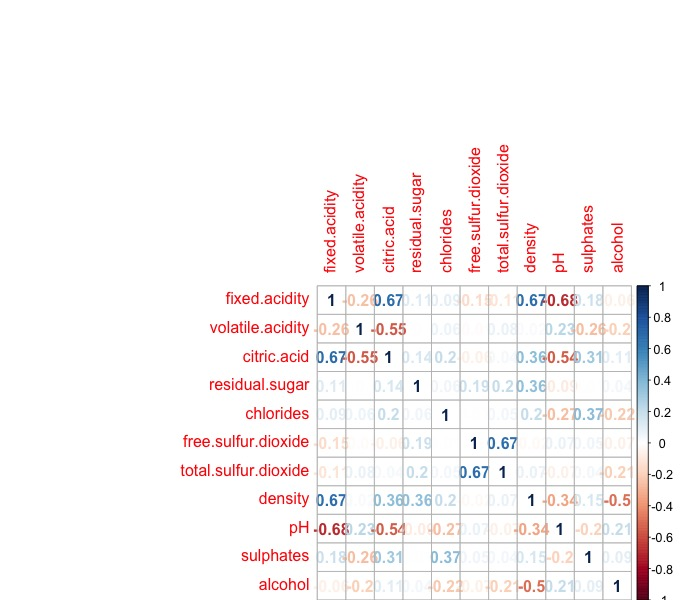
\includegraphics[trim={5cm, 0, 1cm, 1cm}, scale=.3]{corrgram}
	\caption{Correlation matrix of wine quality dataset}
\end{figure}


\section*{2-Wine quality transformation?}
The dependent variable wine quality is measured from 0-10, 10 being the best wine 0 the worst wine. There does not appear to be any reason to transform this variable to anything other than what it is already. A log transformation would require changing the scale slightly to not include 0 and would not change the analysis at all. There would still be 11 distinct categories, only they would be in log's, and would require more work to interpret the results. No other reasonable transformation is necessary.
\section*{3-Acidity measures}
Of the three measures of acidity: fixed acidity, volatile acidity and citric acid the best one to use in this context is volatile acidity. The determination of this came from looking at the correlation matrix of the three variables with the dependent variable quality. The one that explains quality the most would be the one most useful for our analysis. Volatile acidity is correlated with a -0.39 Pearson coefficient while the others are far less. 
\begin{wrapfigure}[11]{r}{0.5\textwidth}
	\includegraphics[scale=.25]{corgram2}
\end{wrapfigure}	
In addition a regression was run with each one of these variables in it as a predictor and quality as the dependent. The $ R^2 $ was then obtained from the output to see which variable did explain the most variation in quality. The results show of $ R^2 $ for regression of quality on fixed acidity, volatile acidity and citric acid were 0.01539, 0.1525, and  0.05124, volatile acidity is the most correlated and has the highest $ R^2 $ in a regression. Therefore, volatile acidity is the variable of the three to use in further analysis.  
	
\section*{4-Sulfates}
	I do not think it makes sense to include only one. For example, free sulphur and sulphates are not correlated (see correlation matrix below) yet they are correlated with quality. To add all three would not make sense because clearly total sulphur dioxide contains much of the information that is in free sulphur dioxide, but it does not make sense to include only one if we are looking for the best explanation of wine quality. 	
\begin{figure}[H]
	\centering
	\includegraphics[scale=.25]{corgram3}
	\caption{Cor. matrix sulphur, sulphates, total sulphur dio.}
\end{figure}	

	
\section*{5-Density}
The median appears to be the best divider between high and low quality wines, about 0.9968. 
\begin{table}[H]
	\centering
	\scalebox{.7}{
\begin{tabular}{cccccc}
	Min. & 1st Quartile & Median & Mean & 3rd Qartile. & Max \\
	\hline 
	0.9901 & 0.9956 & 0.9968 & 0.9967 & 0.9978 & 1.0040 \\
\end{tabular}
}
\caption{Summary statistics for density}
\end{table}
The high quality and low quality wines appear split around this threshold which is observable from the figure below. We would like to split density so that above a certain threshold we observe only high quality wines and below we observe low quality. The best criterion both from the summary statistics and from this plot appear to be the median value.
\begin{figure}[H]
	\centering
	\includegraphics[scale=.25]{densityPlot}
	\caption{Quality (y) vs density (x)}
\end{figure}
	
	
\section*{Forward-Backward-Stepwise Selection}
\begin{enumerate}[label=\alph*)]
	\item Using AIC to search for the best model among the possible 256 models the result was including: Model = volatile.acidity + chlorides +  pH + sulphates + alcohol	
	\item Using BIC to search the result was the same, Model = volatile.acidity + chlorides + pH + sulphates +  alcohol
	\item Using the forward algorithm with a critical value of $ F_{.85, 1, den. df} $ to find the best model the result was the same, Model = alcohol + volatile.acidity + sulphates + chlorides + pH 
	\item Using the backward algorithm with a critical value of $ F_{.85, 1, den. df} $ to find the best model the result was, Model =  volatile.acidity + chlorides + pH + sulphates + alcohol
	\item Using the forward-backward stepwise with an inclusion value of $ F_{.85, 1, den. df} $ and exclusion value of $  F_{.85, 1, den. df} $ the model specified was Model =  volatile.acidity + alcohol + sulphates + chlorides + pH
\end{enumerate}

For the best model the BIC gave the same as AIC in this case, Model = volatile.acidity + chlorides + pH + sulphates +  alcohol. The true model seems to contain at least these five parameters. These five parameters also possibly interact in some way and we consider that next. Putting additional parameters may improve the fit however it will decrease the confidence we have in our estimates so it is a balance. The amount of interactions that are possibly including the parameters that we know we will include brings the total amount of possible parameters up to $ 2^15 $. After examining  the results using the previous methods at least one interaction term seems important. Using a modified backwards elimination method by keeping the variables that survived the previous forwards and backwards elimination steps and only considering a full model with a interaction and a reduced model without the interaction we consider all possible interactions one at a time with the model given above. The results are below:
\begin{table}[H]
	\centering
	\scalebox{.5}{
\begin{tabular}{rl}
	Addition to base model & F-Statistic \\
	\hline 
	volatile acidity $ \times $ chlorides &  0.002 \\
	volatile acidity $ \times  $ free sulphur dioxide & 0.157 \\
	volatile acidity $ \times $ pH & 0.101 \\
	volatile acidity $ \times $ alcohol & 0.815 \\
	chlorides $ \times $ free sulphur dioxide & 4.890 \\
	chlorides $ \times $ pH & 6.882 \\
	chlorides $ \times $ alcohol & 0.206 \\
	free sulphur dioxide $ \times $ pH & 1.667 \\
	free sulphur dioxide $ \times $ alcohol & 1.566 \\
	pH $ \times $ alcohol & 2.333\\
	\hline 
\end{tabular}
}
\caption{All interactions of variables included in the model considered.}
\end{table}

The model that will determine wine quality the best is evidently, \text{Quality} =  \\ \text{ volatile.acidity + alcohol + sulphates + chlorides + pH + chlor.pH}

And the results from R, 
\begin{table}[H]
	\centering
	\scalebox{.55}{
	\begin{tabular}{llllll}
		                 & Estimate & Std. Error & t       & value & Pr(>|t|) \\
		                 \hline
		(Intercept)      & 5.23224 & 0.61233     & 8.545   & $ <2e^{-16} $ & *** \\
		volatile.acidity & -1.05758 & 0.10078    & -10.494 & $ <2e^{-16} $ & *** \\
		chlorides        & -18.47500 & 6.31996 & -2.923 & 0.00351 & ** \\
		pH               & -0.83908 & 0.19857 & -4.226 & 2.52$ e^{-5} $ & *** \\
		sulphates        & 0.91375 & 0.11307 & 8.081 & 1.25$ e^{-15} $ & *** \\
		alcohol          & 0.30985 & 0.01667 & 18.586 & $ <2e^{-16} $ & *** \\
		chlor.pH         & 5.30190 & 2.02105 & 2.623 & 0.00879 & ** \\
		\hline 
	\end{tabular}
}
\end{table}

With the interaction of chlorides and pH included in this model the t-statistic shows that it is statistically significant with a value of 2.623. The critical value (two-sided) is 1.96 and the two sided p-value is 0.00879. Chlorides and pH are important factors to wine quality. Chlorides give wine a salty taste \cite{winSite} and pH if it is high or low give it a acid or tart taste. The Chlorides saltiness balance the pH, and red wine is especially acidic in comparison with other wines \cite{wineMag}. Therefore when there is a lack of chlorides the quality of the wine will be unbalanced and the acidity of the pH will come through more than it should in a well-balanced wine \cite{wineGeek}.  

The estimated parameters give us an idea of what quality a wine will be if we have the above information. An increase in the measure of volatile acidity has a negative effect on wine which is well known \cite{imbibe}. Therefore, the model predicts quality will go down by almost a full point with a measurable increase in volatile acidity. Chlorides also negative impact wine quality and this phenomenon is also well documented in the literature \cite{winSite}. The measuring of chlorides is very fine so the large estimate needs to be interpreted correctly. The average value of chlorides in this dataset is 0.09. Going up 1/100 would give a -1.8 decrease in wine quality, approximately. Sulphates, alcohol and the interaction all resulted in positive factors for wine quality, however, these results must be taken with caution. One could not simply fill a bottle full of alcohol an expect the quality of wine to be a 10. The balance of these elements must be there for a wine to be truly good. However, excesses detectable by qualified sommeliers and perhaps novices would detract from the quality of the wine. The exceptions sulphates and alcohol are probably explained by the fact that sulphates help preserve a wines taste, wines without sulphates frequently spoil and taste terrible \cite{orgainicwine}. In addition, alcohol is stronger in more aged wines and more aged wines generally are regarded as better wines, the flavors having come into more fruition after proper aging. This could explain why more alcohol is generally present in better wines. 

\section*{Model Performance}
The model performed well when the dataset was divided into two distinct groups, a training and a testing set. 90\% of the data was used for a testing set on which the parameters were estimated. The estimated parameters were then used on the validation set data to predict wine quality. The squared average of this vector was taken and the result was 0.483. This error shows the model performs well in fitting the data.

\begin{thebibliography}{9}
	\bibitem{winSite} 
	Marina Sonegheti Coli, Angelo Gil Pezzini Rangel, Elizangela Silva Souza, Margareth Ferraro Oliveira, Ana Cristina Nascimento Chiaradia. 
	\textit{Chloride concentration in red wines: influence of terroir and grape type}. 
	Food Sci. Technol (Campinas) vol.35 no.1 Campinas Jan./Mar. 2015.
	
	\bibitem{wineMag} 
	Daniel Pambianchi. 
	\textit{pHiguring out pH}. 
	\url{https://winemakermag.com/547-phiguring-out-ph}.
	
	\bibitem{wineGeek} 
	Madeline Puckette ,
	\url{http://winefolly.com/review/understanding-acidity-in-wine/}.
	
	\bibitem{imbibe}
	Clinton Cawood. \url{http://imbibe.com/news-articles/wines/senior-judges-swa-wine-faults/}.
	
	\bibitem{orgainicwine}
	\url{http://theorganicwinecompany.com/sulfites-in-wine-facts/}
\end{thebibliography}






\end{document}
